\section{Fluctuations, Continued}

\subsection{Phase and Amplitude Fluctuations}
We consider $\phi$ (the effective Hamiltonian/energy):
\begin{equation}
    \phi(\v{m}) = \frac{\kappa}{2}\abs{(\nabla \v{m})}^2 + \frac{t}{2}m^2 + \frac{u}{4}m^4
\end{equation}
where $\v{m}$ is a order parameter with magnitude $m = \abs{\v{m}(\v{x})}$ but also a phase (as it has a direction).

Looking at the potential, we have massless ``Goldstone'' modes that go between the two wells and the massive modes that oscillate inside of a given well.

\begin{figure}[htbp]
    \centering
    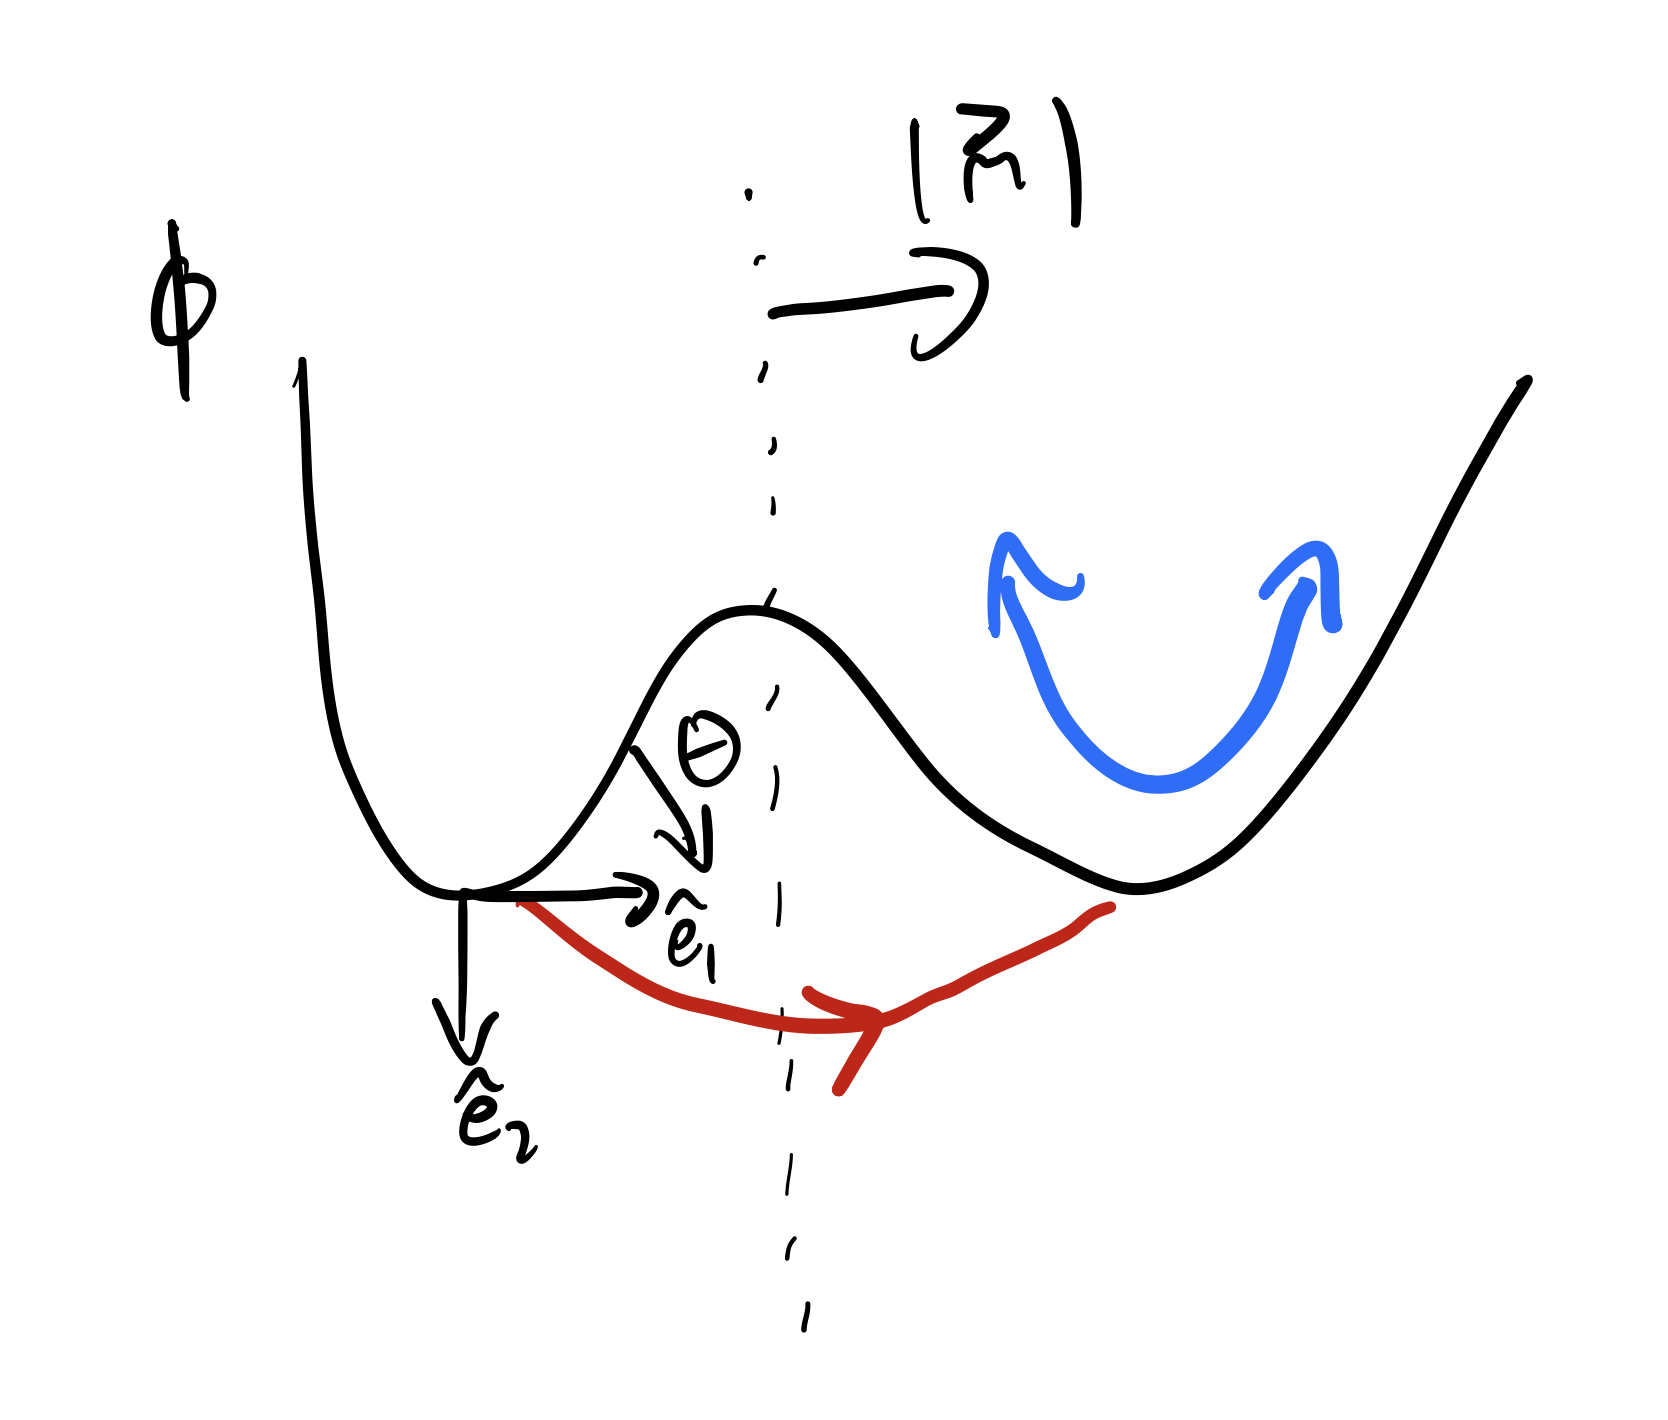
\includegraphics[scale=0.3]{Lectures/Figures/mexican_hat_fluctuations.png}
    \caption{We consider a potential/energy $\phi$ that depends on an order parameter $\v{m}(\v{x})$. The order parameter has magnitude $m = \abs{\v{m}}$ and direction $\theta$. There are massless Goldstone modes (red) that go between the wells of the potential, and massive modes that stay within a potential. For a given direction of the order parameter, we choose locally a coordinate system such that $\hat{e}_1$ points along the direction of magnetization and $\hat{e}_2$ (and other vectors) to be mutually orthogonal. This plot is for $t < 0$.}
    \label{fig:mexican_hat_fluctuations}
\end{figure}

We wish to find the probability distribution:
\begin{equation}
    \mathcal{P}[\v{m}(\v{x})] = \exp(-\int d^dx \phi(\v{m}, \v{x})).
\end{equation}

Let us notate $\avg{m} = \bar{m}$ and then write:
\begin{equation}
    m = [\bar{m} + \phi_l(\v{x})]\hat{e}_1 + \sum_{\alpha=2}^n \phi_{t, \alpha}(\v{x})\hat{e}_\alpha
\end{equation}
Where $\hat{e}_1$ is a vector parallel to the magnetization, and and $\hat{e}_\alpha$ for $\alpha = \set{2, \ldots, n}$ are vectors perpendicular to the magnetization and mutually orthogonal. The $\phi_l, \phi_t$ appearing above are the longitudinal and transverse fluctuations, respectively.

We consider the mean field solution:
\begin{equation}
    \bar{m} = \begin{cases}
    0 & t > 0
    \\ \sqrt{-\frac{t}{u}} & t < 0
    \end{cases}
\end{equation}
Which we then obtain:
\begin{equation}
    -\ln \mathcal{P} = V\left[\frac{t}{2}\bar{m}^2 + \frac{u}{4}\bar{m}^4\right] + \int d^dx \left(\frac{\kappa}{2}\abs{\nabla \phi_l}^2 + \left(\frac{t + 3u\bar{m}^2}{2}\right)\phi_l^2\right) + \int d^dx \left(\frac{\kappa}{2}\abs{\nabla \phi_t}^2 + \left(\frac{t + u\bar{m}^2}{2}\right)\phi_t^2\right) + O(\phi_{l/t}^4)
\end{equation}
Let us rescale:
\begin{subequations}
    \begin{align}
        \frac{\kappa}{\xi_l^2} &= t + 3u\bar{m}^2 = \begin{cases}
            t & t > 0
            \\ -2t & t < 0
        \end{cases}
        \\ \frac{\kappa}{\xi_t^2} &= t + u\bar{m}^2 = \begin{cases}
            t & t > 0
            \\ 0 & t < 0
        \end{cases}
    \end{align}
\end{subequations}
Where the $\xi$ are called correlation lengths. Above the mean-field phase transition they are the same. Below, they are different. The $0$ is the Goldstone mode (gapless, linear) and the $-2t$ is the massive mode (gapped, looks like a harmonic oscillator at long wavelengths).

We now have translation invariance, so a natural change of basis is to go into Fourier/momentum space:
\begin{equation}
    \phi(x) = \sum_\v{q} \phi_\v{q} \frac{e^{i\v{q} \cdot \v{x}}}{\sqrt{V}}
\end{equation}
We then find:
\begin{equation}
    \mathcal{P}[\phi_{l\v{q}}, \phi_{t\v{q}}] \propto \prod_{\v{q}, \alpha}\exp(-\frac{\kappa}{2}\left(\v{q}^2 + \xi_\alpha^{-2}\right)\abs{\phi_{\alpha\v{q}}}^2)
\end{equation}
We can now start to compute objects of interest, e.g. correlation functions (between fluctuations). We call this the structure factor:
\begin{equation}\label{eq:structurefactor}
    S(\v{q}) = \avg{\phi_{\alpha\v{q}}\phi_{\beta\v{q}'}} = \frac{\delta_{\alpha\beta}\delta_{\v{q},-\v{q}'}}{\kappa(q^2 + \xi^2_\alpha)}
\end{equation}
The decoupling of longitudinal/transverse gives the first delta function and the second comes from momentum conservation. The denominator comes from the computation of the Gaussian integrals. Plotted, it looks like:

\begin{figure}[htbp]
    \centering
    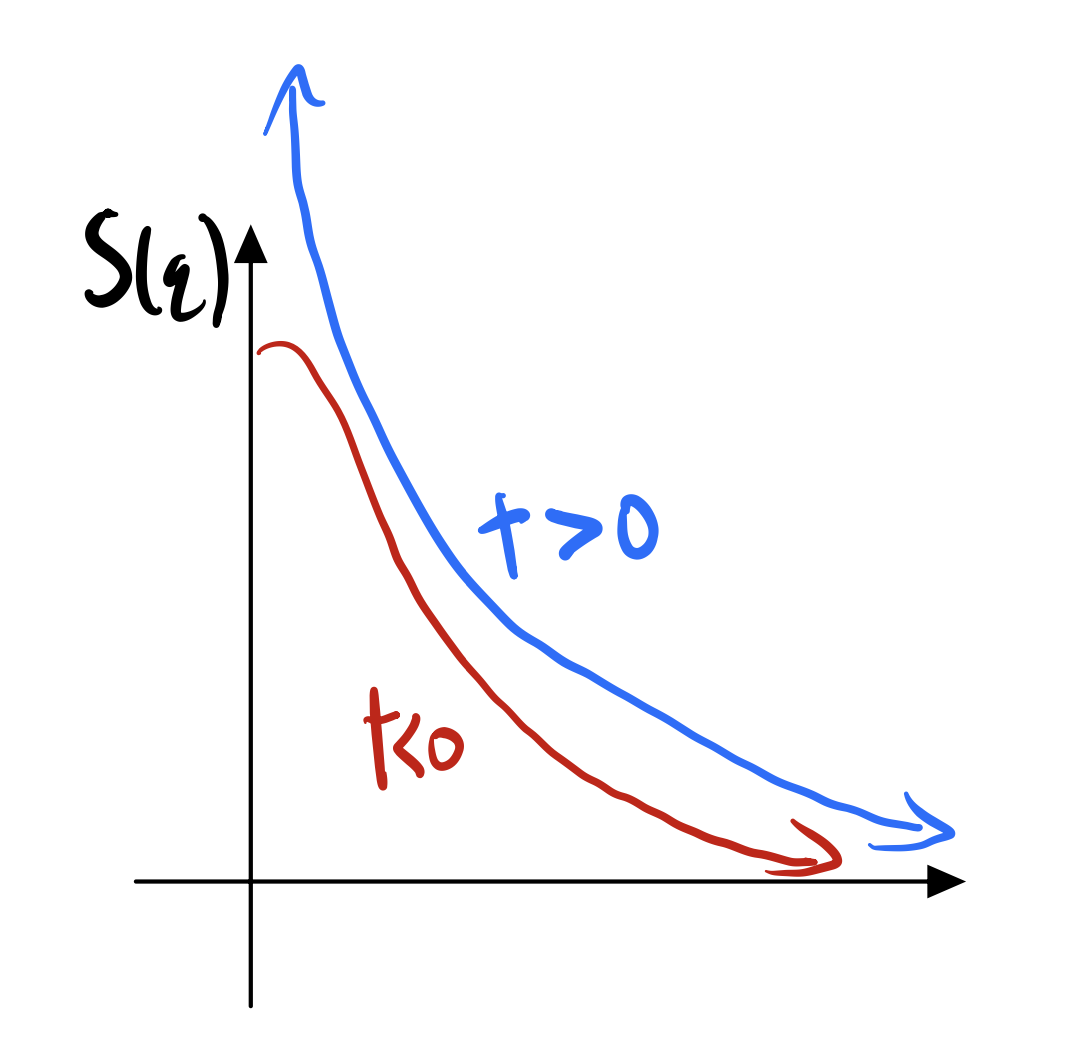
\includegraphics[scale=0.3]{Lectures/Figures/structure_factor.png}
    \caption{Plot of structure for transverse modes as a function of $q$. For $t < 0$ we have $\xi_t = 0$ and so the structure factor diverges at $0$. For $t > 0$, $\xi_t$ is finite so the structure factor at $0$ does not diverge. The structure factor for the longitudinal fluctuations has the same general shape as the $t > 0$ transverse fluctuations (for $t < 0$ and $t > 0$; $\xi_l$ is finite for both regimes, just with a different prefactor. For $t > 0$ it is identical to the transverse fluctuations).}
    \label{fig:structure_factors}
\end{figure}

What is the interpretation of $S(\v{q})$? We have some object of interest, which we probe via a scattering experiment. We have some probe, which could be an electron, neutron, photon etc. It has an incident wavevector $\v{k}_i$ and a output wavevector $\v{k}_f$, emerging at some angle $\theta$ to the incident. If we have elastic scattering, then the energy of the particle remains unchanged, but there is some changed momenta, i.e. $\v{k}_f = \v{k}_i + \v{q}$. We then study the scattering amplitude:
\begin{equation}
    A(q) \propto \bra{\v{k}_f}\v{U}\ket{\v{k}_i} \propto \sigma(\v{q})\int d^dx e^{i\v{q}\cdot \v{x}}\rho(\v{x}) \propto \rho_\v{q}
\end{equation}
Note that the average over the scattering amplitude vanishes:
\begin{equation}
    \avg{A(q)} = \avg{\rho_\v{q}} = 0
\end{equation}
So to probe the structure we want to study:
\begin{equation}
    S(q) = \avg{\abs{A(\v{q})}^2} \propto \avg{\rho_\v{q}}
\end{equation}

\subsection{Technical Aside: Gaussian Integrals}
Consider the single variable integral:
\begin{equation}
    I_1 = \int_{-\infty}^\infty d\phi e^{-\frac{1}{2}k\phi^2 + n\phi}
\end{equation}
We solve via completing the square and then redefinition of the integration variable to $\phi' = \sqrt{k}(\phi - \frac{h}{k})$. What is left with just the familiar Gaussian integral, which we should be familiar with the result of:
\begin{equation}
    I_1 = \int_{-\infty}^\infty d\phi e^{-\frac{1}{2}k(\phi - \frac{h}{k})^2 + \frac{h^2}{k}} = \sqrt{\frac{2\pi}{k}}e^{\frac{h^2}{2k}}
\end{equation}
Now consider $\dod{I_1}{h}$, which via differentiating under the integral sign we know is equivalent to $\avg{\phi}$.
\begin{equation}
    \dod{I_1}{h} = \int d\phi \phi e^{-(\ldots)} = \avg{\phi} = \frac{h}{k}
\end{equation}
This integral is correct up to a constant factor. We don't have to care about these constants, as eventually we take the logarithm of the partition function, and this becomes an additive constant which has no effect on the physics. We can also look at the second derivative:
\begin{equation}
    \dod[2]{I_1}{h} = \avg{\phi^2} = \frac{h}{k} + \frac{h^2}{k^2}
\end{equation}
We can also look at the cumulant:
\begin{equation}
    \avg{\phi^2}_c = \avg{\phi^2} - \avg{\phi}^2 = \frac{h}{k}.
\end{equation}
In principle we could go to higher order cumulants, but you can verify for yourself that these would all vanish.

Now, let's look at the $N$-dimensional version:
\begin{equation}
    I_N = \int_{-\infty}^\infty \prod_{i=1}^N d\phi_i \exp(-\frac{1}{2}\sum_{ij}\phi_i K_{ij}\phi_j + \sum_i n_i \phi_i) = \sqrt{\frac{(2\pi)^N}{\det K}}\exp(\sum_{ij}h_i \frac{K_{ij}^{-1}}{2}h_j)
\end{equation}
How would we obtain this? $K$ is a general, presumably symmetric matrix. We diagonalize $K$, and suppose it has eigenvalues $K_{ij}\hat{q}_j = K_q \hat{q}_j$. We use the $\hat{q}_j$ as the canonical basis, and rotate into this basis by saying $\phi_i = \sum_q \tilde{\phi}_q \hat{q}_i$. Thus the integral becomes:
\begin{equation}
    I_N = \int \prod_{q=1}^N d\tilde{\phi}_q \exp(-\frac{K_q}{2}\phi_q^2 + h_q\tilde{\phi}_q) = \prod_{q=1}^N\sqrt{\frac{2\pi}{K_q}}\exp(h_q\frac{K_q^{-1}}{2}h_q)
\end{equation}
where now recognizing the determinant is just the product of the eigenvalues, and rotating back into the eigenbasis, gives the desired expression.

Remark: This relation is very useful, and it works out for QFTs as well, with some $i$s floating around.

\subsection{Back to Physics - Transverse Fluctuations and Coloumb Emergence}
Now, we make the remark that all Gaussian theories are \emph{solvable} - they may be wrong, but they are solvable. In other words, mean field theory + fluctuations to lowest order (i.e. quadratic) are completely solvable analytically, and are known as Gaussian theories. They are simple, but already can give us interesting phenomena.

For example, for the structure factors appearing in Eq. \eqref{eq:structurefactor}, we were able to find this just with a Gaussian theory, and it tells us that the long wavelength/small $q$ is the interesting regime where things are happening. We can look at the exponent $\eta$ that tells us how the structure factor scales.
\begin{equation}
    S(q, t=0) \sim \frac{1}{q^{2 - \eta}}
\end{equation}

Let us focus on the tranverse fluctuations, below the critical temperature, so $t < 0$ with $\eta_t = 0$. Then, we have:
\begin{equation}
    \mathcal{P}(\Theta(q)) \propto \exp(-\frac{\kappa}{2}\sum_q q^2\abs{\Theta_q}^2)
\end{equation}
So with out computed structure factor, let us look at the probability fluctuations in the angles:
\begin{equation}
    \avg{\Theta_\v{q}\Theta_{\v{q}'}} = \frac{\delta_{\v{q} + \v{q}'}}{\kappa q^2}
\end{equation}
Going back into real space, this is the statement that:
\begin{equation}
    \avg{\Theta(\v{x})\Theta(\v{x}')} = \frac{1}{V}\sum_\v{q}e^{i\v{q}(\v{x} - \v{x}')}{\kappa q^2} = \int \frac{d^dq}{(2\pi)^d}\frac{e^{i\v{q}\cdot(\v{x} - \v{x}')}}{q^2}
\end{equation}
This is just the Coloumb potential:
\begin{equation}
    C(\v{x}) = -\int \frac{d^d q}{(2\pi)^d}\frac{e^{i\v{q}\cdot\v{x}}}{q^2}
\end{equation}
Which satisfies $\nabla^2 C = \delta^d(\v{x})$, i.e. just Gauss' Law for a point charge. Now, we can ask what happens to the potential as $x \to \infty$?
\begin{equation}
    \lim_{x \to \infty}C(x) \propto \begin{cases}
        \text{Const} & d > 0
        \\ x^{2-d} & d < 2
        \\ \ln(x) & d =2 
    \end{cases}
\end{equation}
This behaviour can be obtained by looking at $d^dq \sim q^{d-1}dq$ (plus various angular integrals which we don't care about). 

Thus, in low dimensions the correlations fall off like a power law, so no long range order. For $d > 2$ we maybe have LRO. At $d = 2$, we have the critical/marginal dimension. We have a pesky logarithm, and we need more work (which we will study in future lectures).

Earlier on, we explained how there were models (AFM Heisenberg) that did not order at low dimensions due to the presence of soft modes. This is a souped up version of that. So, when generally looking at a theory, if I look at a theory with Goldstone modes, I should look at the phase fluctuations and see if I get LRO. Even though in principle the length scales can get very large, we can still say that at very large scales that the correlations fall off. Also, its worth noting that the LRO is temperature dependent; we dropped the $\beta$s through the calculations here, but it is relevant.